\documentclass[a4paper,12pt]{report}
\usepackage{mypackage}


\title{Electrodynamics}

\author{Haydn Cheng}

\date{}

\begin{document}
	\maketitle
	\tableofcontents
	
	\chapter{Electrostatics}
	\section{Electric Field and Potential}
	\todo{problem 1.16, 1.39}
	
	Any high school student would say that the electric field created by a point charge \(Q\) is given by
	
	\begin{equation}
		\vb{E} = \frac{Q}{4\pi \epsilon_0r^2} 
	\end{equation}
	
	In this set of notes, we adopt the notation used in Griffiths(3rd ed.), where \(\vb{r}\)  denotes the vector pointing from the origin to a point in space, \(\vb{r}'\) denotes the position vector of the source of electric or magnetic field and \(\brcurs = \vb{r} - \vb{r}'\) denotes the displacement vector pointing from the source to the point in space and \(\rcurs = \left| \brcurs  \right| = \left| \vb{r} -\vb{r} ' \right|  \). With this notation, the electric field created by a known charge distribution \(\rho (\vb{r}')\)  is given by: \footnote{since \(\hrcurs \) is inside the integral sign, in practice we must work with Cartesian coordinates and take \(\vb{x}, \vb{y} \text{ and } \vb{z} \) out of the integral before performing the integral even if we use \(r, \theta \text{ or } \phi\) as variables. So we sum over the field component (along \(\vb{x}, \vb{y} \text{ or } \vb{z}\)) (usually by multiply something like \(\cos \alpha\) of infinitesimal sources, where \(\alpha \) can be expressed in terms of \(r, \theta \text{ or } \phi\).}
	
	\begin{equation}
		\vb{E}(  \vb{r}) = \frac{1}{4\pi \epsilon_0} \int \frac{\rho ( \vb{r}' ) }{\rcurs ^2}  \hrcurs d\tau '. \label{comb} 
	\end{equation}
	
	Here \(\rho \) is a function of \(\vb{r}'\) instead of \(\vb{r}\) since \(\vb{r}\) is just an arbitrary point in space. Accordingly, the infinitesimal volume \(d\tau '\) is primed. If no confusion would arose, the prime notation is usually omitted.
	
	Taking the divergence of \cref{comb}, we have 
	\begin{equation}
		\div{\vb{E}} = \frac{1}{4\pi\epsilon_0} \int \div{\frac{\hrcurs }{\rcurs ^2} } \rho (\vb{r} ')d\tau '. 	 
	\end{equation}
	
	In Maths notes, we have proved that 
	\begin{equation}
		\div{\frac{\hrcurs }{\rcurs ^2} } = 4\pi \delta ^3 ( \brcurs  ) .
	\end{equation}
	
	So, we yield the Gauss's Law in differential form
	\begin{equation}
		\div{\vb{E} ( \vb{r}  ) }  = \frac{1}{4\pi\epsilon_0} \int 4\pi \delta ^3 ( \vb{r} -\vb{r} ' ) \rho ( \vb{r} ' ) d\tau ' = \frac{\rho ( \vb{r})  }{\epsilon_0}. \label{divE} 
	\end{equation}
	
	Taking the curl of \cref{comb},
	\begin{equation}
		\curl{\vb{E} } = \frac{1}{4\pi\epsilon_0} \curl{\int \frac{\hrcurs }{\rcurs ^2} \rho d\tau } = \frac{1}{4\pi\epsilon_0} \int \rho (\curl{\frac{\hrcurs }{\rcurs ^2}}) d\tau = 0. \label{curlE} 
	\end{equation}
	
	Here \(\rho \) is taken outside the curl because \(\rho \) depends on \(\vb{r} '\) but not \(r\) and we invoked the fact that \(\curl{(\frac{\hrcurs }{\rcurs ^2}) } = 0\) which is trivial since the vector field point radially outwards at every point, so it has spherical symmetry.
	
	According to the Helmholtz theorem proved in Maths, we can define a scalar function \(V(\vb{r} )\) which satisfies
	
	\begin{equation}
		\vb{E} (\vb{r} ) = -\grad{V(\vb{r}) } \label{gradV} 
	\end{equation}
	
	and 
	
	\begin{equation}
		V(\vb{r} ) = \frac{1}{4\pi\epsilon_0} \int \frac{\rho (\vb{r} ')}{\rcurs } d\tau '. \label{potential} 
	\end{equation}
	
	
	Integrating both sides of \cref{gradV} and utilizing the fundamental theorem for gradients, we have 
	\begin{equation} 
		\begin{aligned}
			-\int_{\vb{a} }^{\vb{b} } \vb{E} \cdot d\vb{l} &= \int_{\vb{a} }^{\vb{b} } (\grad{V} ) \cdot d\vb{l} \\
			V(\vb{b} ) - V(\vb{a} ) &= -\int_{\vb{a} }^{\vb{b} } \vb{E} \cdot d\vb{l} \\
			&= -\int_{\vb{O} }^{\vb{b} } \vb{E} \cdot d\vb{l} - \int_{\vb{a} }^{\vb{O}} \vb{E} \cdot d\vb{l} 
		\end{aligned}
	\end{equation}
	
	where \(\vb{O} \) is some arbitrary reference point.
	
	Since \(\vb{a} \text{ and }  \vb{b} \) are arbitrary points, the terms that depends on \(\vb{a} \) on the left hand side of the equation must be identical to the terms that depends on \(\vb{a} \) on the right hand side of the equation (and the same holds for \(\vb{b} \) ). So we have an explicit formula for the electric potential \(V(\vb{r} )\) 
	
	\begin{equation}
		V(\vb{r} ) = -\int_{\vb{O} }^{\vb{r} } \vb{E} \cdot d\vb{l} . 
	\end{equation}
	
	Note that although this definition of \(V(\vb{r} )\) involves a path integral, the value of \(V(\vb{r} )\) is well defined and path independent as guaranteed by the Helmholtz theorem.
	
	Also, we see that the electric potential \(V(\vb{r} )\) only makes sense with reference to a point. So only the difference in potential of two points is a unique value. Usually, we take this reference point to the infinity. It so happens that the \(V(\infty)\) is zero because it is away from all charges.\footnote{In cases where the charge distribution itself extends to infinity, such as an infinite charged wire, the potential blows up so we will have to redefine the reference point.} However, no matter where the reference point is taken, the electric field is not affected since \(\boldsymbol{\nabla}(\vb{r} ) = \grad{(V(\vb{r} ) + K)} - \grad{V(\vb{r} )} = \vb{E} (\vb{r} )\).
	
	
	So with this potential formulation in hand, we see that there are two fundamental ways to calculate the electric field: the first is directing summing over the electric field by Coulomb's law by \cref{comb}, and this includes applying Gauss's law in integral form whenever symmetries are present. The second way to first calculate the potential by \cref{potential} then take the gradient of it. Sometimes, one is more simpler than the other.
	
	
	A diagram illustrating the relations between \(\rho , V \text{ and } \vb{E} \) is shown in \cref{relations}. \onefig{relations}{scale=0.2} 
	
	\begin{example_template}
		\textbf{Example:} \textbf{Griffths 5rd ed. Problem 2.56} \newline \newline
		\textbf{Question:} Find the charge density for the electric field \(\vb{E} = ax \vu{x} \)
		\newline \newline
		\textbf{Solution:}  \(\rho = \epsilon_0 \div{\vb{E} } = \epsilon_0 a\). However, the same charge density would also be compatible with \(\vb{E} = ay \vu{y} \text{ or } \vb{E} = \frac{a}{3} \vu{r} ...\) The crucial insight is that the curl and divergence of  \(\vb{E} \) don't determine the field uniquely. They must be supplemented by appropriate boundary conditions. In the ordinary cases mentioned in the Helmholtz theorem, we impose the boundary condition that \(\vb{E}\) goes to zero as \(r \rightarrow \infty\). When the charge distribution doesn't converge, we have to rely on symmetries to ensure that the electric field is uniquely determined. For example, the magnitude of electric field must be the same on both sides of an infinite plane of surface charge. In this case, however, there are no natural boundary conditions nor persuasive symmetries. So the field is not uniquely determined or there are not sufficient conditions to determine the answer.
		
		
		
		
		
		
	\end{example_template}
	
	
	
	
	\section{Energy}
	From the energy-work-theorem, we know that 
	
	\begin{equation}
		\Delta W = \Delta K.
	\end{equation}
	
	So to move a charge \(Q\) from \(\vb{a} \) to \(\vb{b} \), an external work \(W_{me} \) has to be done which satisfies
	
	\begin{equation}
		W = W_{me} + W_{electric} = W_{me} + Q \int_{\vb{a}  }^{\vb{b} } \vb{E} \cdot d\vb{l} =  W_{me} + Q(V(\vb{b} ) - V(\vb{a} )) = 0.
	\end{equation}
	
	Therefore, we have 
	
	\begin{equation}
		W_{me}  = Q(V(\vb{b} ) - V(\vb{a} )) .
	\end{equation}
	
	If the beginning and end points are infinity and \(\vb{r} \) respectively, then
	
	\begin{equation}
		W_{me}  = QV(\vb{r} )
	\end{equation}
	
	So \(QV\) is both work done by external force and the potential energy of the charge. An important point to note is that \(V\) here is the potential created by other charges that already exist before we bring in the charge that we are considering.
	
	
	For a pair of point charges, the work done required and the potential energy is (since the first charge can be bring to its position without any energy requirement)
	
	\begin{equation}
		U = W_{me} = \frac{1}{4\pi\epsilon_0} \frac{Qq}{\rcurs } . \label{energy1} 
	\end{equation}
	
	
	Therefore, the work done to assemble a collection of charges, or the potential energy possessed by a group of charges will be
	
	\begin{equation}
		U = W_{me} = \frac{1}{4\pi\epsilon_0} \sum_{i=1}^{n} \sum_{j>i}^{n} \frac{q_{i} q_{j} }{\rcurs _{ij} }  = \frac{1}{2} \frac{1}{4\pi\epsilon_0} \sum_{i=1}^{n} \sum_{j\neq i}^{n} \frac{q_{i} q_{j} }{\rcurs _{ij} } = \frac{1}{2} \sum_{i=1}^{n} q_{i} \sum_{j\neq i}^{n} \frac{1}{4\pi\epsilon_0} \frac{q_{j} }{\rcurs _{ij} } = \frac{1}{2} \sum_{i=1}^{n} q_{i} V(\vb{r} '). \label{energy2} 
	\end{equation}
	
	For continuous charge distribution, the work done required or the energy of the system becomes
	
	\begin{equation}
		U = W_{me} = \frac{1}{2} \int \rho V d\tau. \label{energy3} 
	\end{equation}
	
	An equally important point to note here is the \(V\) here doesn't have any ambiguity since the contribution of \(dq = \rho  d\tau \) can be neglected.
	
	
	
	Since \(\rho  = \epsilon_0 \div{\vb{E} } \), so 
	
	\begin{equation}
		\begin{aligned}
			U = W_{me} &= \frac{\epsilon_0}{2} \int (\div{\vb{E}} ) V d\tau \\ &= \frac{\epsilon_0}{2} (-\int_{\mathcal{V} } \vb{E} \cdot (\grad{V} ) d\tau + \oint_{\mathcal{S} }  V\vb{E} \cdot d\vb{A}) \\ &= \frac{\epsilon_0}{2} (\int_{\mathcal{V} }  E^2 d\tau + \oint_{\mathcal{S} }  V\vb{E} \cdot d\vb{A} ) . \label{energy4} 
		\end{aligned}
	\end{equation}
	
	As long as the volume we use enclose all the charges, we will obtain the correct work done or potential energy from \cref{energy2}, just that the contribution of the two terms will be different. So, taking the volume to be all space, we have 
	
	\begin{equation}
		U = W_{me} = \frac{\epsilon_0}{2} \int_{all \text{ } space}  E^2 d\tau \label{energy5} 
	\end{equation}
	
	Since the surface integral goes to zero as \(r \rightarrow \infty\).
	
	We see that there are two fundamental ways to compute the work done to assemble a system or the potential energy of a system: the first is to directly calculate the interaction between charges either by considering their assembly process or from the final configuration from \cref{energy3} and the second way is to calculate the energy stored in the electric field created by these charges from \cref{energy4}. \footnote{Here and after, I will refer to \emph{work done to assemble the system or the potential energy possessed by the system} with just \emph{potential energy of the system.}}
	
	From \cref{energy1}, we can see that the energy of a system can be negative as long as there are opposite charges. However, from \cref{energy5}, the energy of a system can only be a positive number. 
	
	This discrepancy arises because in \cref{energy1} we did not calculate the energy required to make the point charges themselves but concerned in the work done required in moving these point charges around. They indeed exist (which one can think of is the energy stored in its radially outward electric field) and are not negligible (in fact, if we try to calculate them, with \cref{energy5}, the result blows up to infinity due to the singularities located at the centers of the point charges.). 
	
	In \cref{energy5}, however, the \emph{point charges} (\(dq = \rho d\tau \))
	are negligible when compared to the charges that already exist beforehand, thus it tells us the total potential energy stored in a charge configuration.
	
	So for artificial problems that involves point charges, it is better to stick with \cref{energy2} while for real-world problems \cref{energy3} is the way to go.
	
	\begin{example_template}
		\textbf{Example:} \textbf{Griffths 5rd ed. Problem 2.38} \\ \\
		\textbf{Question:} Calculate the energy of the system consisting of a point charge \(q_1\) located at the origin and \(q_2\) located at \( z=a \) which \cref{energy5} .  \\ \\
		\textbf{Solution:}  A high school student would tell you that the energy is \(\frac{1}{4\pi\epsilon_0} \frac{q_1q_2}{a} \) which is indeed correct. However, deriving this result with  \cref{energy5} requires more careful treatments. The total electric field \(\vb{E} \) is the sum of the electric fields of two individual charge
		\begin{equation}
			\vb{E} = \vb{E} _{1} + \vb{E} _{2} = \frac{1}{4\pi\epsilon_0} \frac{q_1}{r^2} \vu{r} + \frac{1}{4\pi\epsilon_0} \frac{q_2}{\rcurs ^2} \hrcurs. 
		\end{equation}
		So from \cref{energy5}, we have 
		\begin{equation}
			U = W_{me} = \frac{\epsilon_0}{2} \int _{all \text{ } space} \left| \vb{E} _{1} + \vb{E} _{2}  \right| ^2 d\tau = \frac{\epsilon_0}{2} \int _{all \text{ } space} (\left| \vb{E} _{1}  \right| ^2 + \left| \vb{E} _{2}  \right| ^2 + 2\left| \vb{E} _{1} \cdot \vb{E} _{2}  \right|) d\tau .
		\end{equation}
		The first two terms in the integrand are precisely the energy possessed by the charges themselves which we blow up. Therefore,
		
		\begin{equation}
			U = \epsilon_0 (\frac{1}{4\pi\epsilon_0} )^2 \int_{0}^{\infty} \int_{0}^{\pi } \int_{0}^{2\pi }     \frac{1}{r^2\rcurs ^2} \cos \beta r^2\sin \theta drd\theta d\phi 
		\end{equation}
		where \(\beta \) is the angle between \(\brcurs \text{ and } \vb{r} \text{ which equals to } cos^{-1} \frac{r-a \cos \theta }{\rcurs }  \) and \(\rcurs = \sqrt{r^2 + a^2 -2ra\cos \theta } \). So the integral becomes
		
		\begin{equation}
			2\pi \epsilon_0 (\frac{1}{4\pi\epsilon_0} )^2 \int_{0}^{\infty} \int_{0}^{\pi } \frac{r-a \cos \theta }{\rcurs ^3} \sin \theta drd\theta  
		\end{equation}
		
		which can be showed to be identical to \(\frac{1}{4\pi\epsilon_0} \frac{q_1q_2}{a} \) which verify our \emph{point charge} approach.	
	\end{example_template}
	
	\begin{example_template}
		\textbf{Example:} \textbf{Griffths 5rd ed. Problem 2.61} \newline \newline
		\textbf{Question:} Find the energy required to move a point charge  \(q\) from the center of a conducting spherical shell with inner radius \(a\) and outer radius \(b\) to infinity.
		\newline \newline
		\textbf{Solution:} We know that the energy of the system in its final configuration is zero, as there is only one point charge at infinity and a conductor with no net or induced charge. Note that the initial charge configuration consists of a point charge \(q\) at the origin, a spherical shell with charge \(-q\) and radius \(a\) and a spherical shell with charge \(q\) and radius \(b\) which encompasses both point charge and uniformly distributed charge so we have to be careful in what \(V\) we use in our calculation.
		
		For the point charge, the potential at the origin is 
		
		\begin{equation}
			V_{point} = \frac{1}{4\pi\epsilon_0} \frac{-q}{a} + \frac{1}{4\pi\epsilon_0} \frac{q}{b}  = \frac{q}{4\pi \epsilon_0} (\frac{1}{b} - \frac{1}{a} )
		\end{equation}
		
		where we excluded the contribution to the potential at the origin by the point charge itself since it blows up and it should not be included anyways.
		
		For the inner shell, the potential at \(a\) is
		
		\begin{equation}
			V_{a} = \frac{1}{4\pi\epsilon_0} \frac{q}{a} + \frac{1}{4\pi\epsilon_0} \frac{-q}{a}  + \frac{1}{4\pi\epsilon_0} \frac{q}{b} = \frac{q}{4\pi \epsilon_0 b} 
		\end{equation}
		
		where the contribution by the inner shell itself is also taken into account because the inner shell is not point charge, so we should use the full potential since individual charges in the inner shell indeed interact with each other.
		
		Similarly, for the outer shell, the potential at \(b\) is
		
		\begin{equation}
			V_{b} = \frac{1}{4\pi\epsilon_0} \frac{q}{b} + \frac{1}{4\pi\epsilon_0} \frac{-q}{b} + \frac{1}{4\pi\epsilon_0} \frac{q}{b}  = \frac{q}{4\pi \epsilon_0 b}   
		\end{equation}
		
		Combining the results, we have 
		
		\begin{equation}
			U_{i} = \frac{1}{2} (q\frac{q}{4\pi \epsilon_0} (\frac{1}{b} - \frac{1}{a} ) + (-q)\frac{q}{4\pi \epsilon_0 b} + q \frac{q}{4\pi \epsilon_0 b}) = \frac{q^2}{8\pi \epsilon_0} (\frac{1}{b} - \frac{1}{a} ) 
		\end{equation}
		
		Thus the work done by the external agent is
		
		\begin{equation}
			W = \Delta U = U_{i} - U_{f} = U_{i} = \frac{q^2}{8\pi \epsilon_0} (\frac{1}{a} - \frac{1}{b} ) .
		\end{equation}
		
		An alternative way to derive this result is to use \cref{energy5}, since we know that the difference in the electric field pattern between the initial and the final state is in the region of the conductor, where the electric field is zero in the former case when compare to \(\frac{1}{4\pi\epsilon_0} \frac{q}{r^2} \) in the latter case, so the energy require to reconstruct this electric field is 
		
		\begin{equation}
			W = \int_{a}^{b} (\frac{1}{4\pi\epsilon_0} \frac{q}{^2} )^2 4\pi r^2dr =   \frac{q^2}{8\pi \epsilon_0} (\frac{1}{a} - \frac{1}{b} ) .
		\end{equation}
		
		An incorrect way to compute this would be to consider the assembly process, since the point charge can be brought to the origin without any work done, the inner shell can be brought in with the work done \(W = \frac{1}{4\pi\epsilon_0} \frac{q^2}{a} \) and the outer shell can be brought in again without any work done since the electric field of the point charge and the inner shell cancel each other out in the region \(r > a\), so it seems like the work done required is \(\frac{q^2}{4\pi \epsilon_0 a} \). However, the defect of this argument is that while it is true that it requires a work done of \(W = \frac{1}{4\pi\epsilon_0} \frac{q^2}{a} \) to move a point charge from infinity to \(a\) in the vicinity of the point charge at the origin, it requires energy to spread them out to a spherical shell, since the spherical shell is no longer an equipotential surface after adding the second point charge.	
	\end{example_template}
	
	
	\section{Conductors}
	To minimize system's energy, free charges on a conductor always resides on the surface, so \(\rho  = \vb{E}  = 0 \) inside the conductor. By considering a Gaussian pillbox on an infinitesimal surface on the conductor, we find that 
	\begin{equation}
		\vb{E} = \frac{\sigma }{\epsilon_0} \vu{n}. 
	\end{equation}
	The electric field is always perpendicular to the surface and the tangential component is zero, thus the surface of the conductor is an equipotential surface which makes sense else charge would experience electric force due to the gradient of electric potential.
	
	Since \(\vb{E} = -\pdv{V}{n} \) (because \(\vb{E} \mathbin{\!/\mkern-5mu/\!} \vu{n} \) at the surface), we have 
	\begin{equation}
		\sigma  = -\epsilon_0 \pdv{V}{n} 
	\end{equation}
	
	In cases where the electric field is discontinuous across surface charges, the force exerted on a patch of charge should be computed by taking the average of the two electric fields. Since
	\begin{equation}
		\vb{E} _{below} = \vb{E} _{patch, below} + \vb{E} _{other}
	\end{equation}
	
	and 
	
	\begin{equation}
		\vb{E} _{above} = \vb{E} _{patch, above} + \vb{E} _{other} 
	\end{equation}
	
	and we also know that 
	
	\begin{equation}
		\vb{E} _{patch, below} = - \vb{E} _{patch, above} = \frac{\sigma }{2 \epsilon_0} \vu{n}  
	\end{equation}
	
	from Gauss's law, we have 
	
	\begin{equation}
		\vb{E} _{other} = \frac{1}{2} ( \vb{E} _{below} + \vb{E} _{above} )
	\end{equation}
	
	In the case of conductor, the force per unit area can be calculated via
	
	\begin{equation}
		\frac{F}{A} = \frac{Q}{A} \frac{1}{2} (0 + \frac{\sigma }{\epsilon_0}) \vu{n}  = \frac{\sigma ^2}{2 \epsilon_0} \vu{n}
	\end{equation}
	
	regardless of the external electric field, because this information is embedded in the fact that \(\vb{E} = 0\) inside the conductor and \(\sigma \) will increase so as to counteract the increasing external field to satisfy this condition.
	
	A capacitor is a fancy word for \emph{a collection of conductors}. Since we know that \(V \propto \rho \propto Q\) from \cref{potential} , we can define the capacitance of a capacitor as
	
	\begin{equation}
		C = \frac{Q}{V} 	
	\end{equation}
	
	where \(V\) is the potential difference between 2 conductor or the potential difference between a conductor compare to infinity. For three or more conductor, there is no trivial definition for the capacitance.
	
	\begin{example_template}
		\textbf{Example:} \textbf{Griffths 5rd ed. Problem 2.43} \newline \newline
		\textbf{Question:} Find the net force that the southern hemisphere of a spherical shell with radius \(R\) and charge \(Q\) exerts on the northern hemisphere.  \newline \newline
		\textbf{Solution:}  Consider the northern hemisphere as a single object, the force that it experiences must be exerted by the southern hemisphere (since there are only 2 objects in play). By symmetry, the force that it experiences must be on its symmetric axis, so the force is 
		
		\begin{equation}
			\int_{0}^{\frac{\pi }{2} } \int_{0}^{2\pi } \frac{\sigma ^2}{2 \epsilon_0} \cos \theta R^2 \sin \theta d\theta d\phi = \frac{Q^2}{32 \pi R^2 \epsilon_0}   
		\end{equation} \label{jk}
		
	\end{example_template}
	
	
	\begin{example_template}
		\textbf{Example:} \textbf{Griffths 5rd ed. Problem 2.48} \newline \newline
		\textbf{Question:} Find the net force that the southern hemisphere of a uniformly sphere with radius \(R\) and charge \(Q\) exerts on the northern hemisphere. \newline \newline
		\textbf{Solution:}  With the same argument as the previous question, the force is
		
		\begin{equation}
			\int_{0}^{R} \int_{0}^{\pi } \int_{0}^{2\pi }    \rho r^2\sin \theta drd\theta d\phi  \frac{1}{4\pi\epsilon_0} \frac{Q\frac{r^3}{R^3} }{r^2} \cos \theta = \frac{3Q^2}{64\pi R^2 \epsilon_0}	\end{equation}
		
	\end{example_template}
	
	\begin{example_template}
		\textbf{Example:} \textbf{Griffths 5rd ed. Problem 2.58} \newline \newline
		\textbf{Question:} For an conducting ellipsoid with total charge \(Q\)
		
		
		\begin{equation}
			\frac{x^2}{a^2} + \frac{y^2}{b^2} + \frac{z^2}{c^2} =1, 
		\end{equation}
		
		the surface charge density can be explicitly calculated as 
		
		\begin{equation}
			\sigma = \frac{Q}{4\pi abc} (\frac{x^2}{a^4} + \frac{y^2}{b^4} + \frac{z^2}{c^4} )^{-\frac{1}{2} }. 
		\end{equation}
		
		By taking appropriate limits, find  \newline a) \(\sigma (r)\) on a circular disk of radius \(R\), \newline b) \(\sigma (x)\) on an infinite sheet which straddles the \(y\)-axis from \(x = -a \) to \(x = a\) in terms of \(\Lambda \) which as the charge per unit length and \newline c) \(\lambda (x)\) on a conducting needle running from \(x = -a \) to \(x = a\). 
		\newline \newline
		\textbf{Solution:}  Using the equation of ellipsoid to eliminate \(z\), we have
		
		\begin{equation}
			\sigma = \frac{Q}{4\pi ab} (c^2(\frac{x^2}{a^4}) + c^2(\frac{y^2}{b^4} ) + 1 - \frac{x^2}{a^2}  - \frac{y^2}{b^2} )^{-\frac{1}{2} }   
		\end{equation}
		
		a) Take \(a = b = R\) and \(c = 0\) such that \(z = 0\) in order to keep \(\frac{z^2}{c^2} \) finite. Then since \(r^2 = x^2 + y^2\), so 
		
		\begin{equation}
			\sigma (r) = \frac{Q}{2\pi R\sqrt{R^2-r^2} }.
		\end{equation}
		
		b) Take \(c = 0\) and let \(\frac{Q}{2b} = \Lambda \), and take the limit \(b \rightarrow \infty\), so
		
		\begin{equation}
			\sigma (x) = \frac{\Lambda }{2\pi \sqrt{a^2 - x^2} } .
		\end{equation}
		
		c) Let \(b = c\) such that the ellipsoid is symmetric about \(x\)-axis and let \(r^2 = y^2 + z^2\). Then
		
		\begin{equation}
			\frac{x^2}{a^2} + \frac{r^2}{c^2} = 1 \label{eps} 
		\end{equation}
		
		and 
		
		\begin{equation}
			\sigma = \frac{Q}{4\pi ac^2\sqrt{\frac{x^2}{a^4} + \frac{r^2}{c^4} } } 
		\end{equation}
		
		Differentiating \cref{eps}, we have 
		
		\begin{equation}
			\dv{r}{x} = -\frac{c^2x}{a^2r}.
		\end{equation}
		
		So
		
		\begin{equation}
			ds = \sqrt{dx^2+dr^2} = dx \sqrt{1+(\dv{r}{x} )^2} = dx \sqrt{1+\frac{c^4x^2}{a^4r^2} } = dx \frac{c^2}{r} \sqrt{\frac{x^2}{a^4} + \frac{r^2}{c^4} } . 
		\end{equation}
		
		Thus
		
		\begin{equation}
			\lambda (x) = \dv{q}{x} = \frac{\frac{Q}{4\pi ac^2\sqrt{\frac{x^2}{a^4} + \frac{r^2}{c^4} } } 2\pi r dx \frac{c^2}{r} \sqrt{\frac{x^2}{a^4} + \frac{r^2}{c^4} } 
			}{dx} = \frac{Q}{2a} .
		\end{equation}
		
		We see that the result is independent of \(c\), so we can take any value of \(c\). In the case of a needle, \(c \rightarrow  0\), and \(\lambda (x)\) is a constant value.
		
		
		
		
		
		
		
		
		
		
		
	\end{example_template}
	
	
	
	
	
	
	
	
	
	
	
	
	
	
	
	
	
	
	
	
	
	
	
	
	
	
	
	
	
	
	
	
	
	
	
	
	
	
	
	
	
	
	
	
	
	
	
	
	
	
	
	
	
	
	
	
	
	
	
	
	
	
	
	
	
	
	
	
	
	
	
	
	
	
	
	
	
	
	
	
	
	
	
	
	
	
	
	
	
	
	
	
	
	
	
	
	
	
	
	
	
	
	
	
	
	
	
	
	
	
	
	
	
	
	
	
	
	
	
	
	
	
	
	
	
	\chapter{Laplace's and Poisson's Equation}
	\section{Uniqueness Theorems}
	\todo{2.5.2 ,ex3.1}
	
	Combining the divergence and curl of electric field (\cref{divE,curlE}), we constructs the Poisson equation
	
	\begin{equation}
		\laplacian V = \frac{\rho }{\epsilon_0}.
	\end{equation}
	
	\(\rho \) equals to zero when we are finding \(V\) outside of the charges, then we have the Laplace's equation
	
	\begin{equation}
		\laplacian V = 0.
	\end{equation}
	
	The Laplace's equation can be visualized by picturing a thin rubber sheet stretched over a cardboard box with wavy boundaries and top part removed (\cref{laplace}). If we lay out coordinates \((x,y)\) on the bottom of the box, the height \(V(x,y)\) of the sheet will satisfy the Laplace's equation (as long as the surface does not deviate too radically from a plane. \onefig{laplace}{scale=0.4} 
	
	From this analog, we see that the value of \(V\) at point \((x,y)\) is the average of those around the point. More precisely, if one draws a circle of any radius \(R\) about the point \((x,y)\), the average value of \(V\) on the circle is equal to the value at the center. Mathematically, 
	
	\begin{equation}
		V(x,y) = \frac{1}{2\pi R} \oint _{circle} Vdl.
	\end{equation}
	
	Consequently, \(V\) has no local maxima or minima for the fact that for an extrema to occur, the surrounding points must all be larger or smaller than the extrema point. However, since the solution of the Laplace's equation is an averaging function, this cannot happen. As a result, all maxima or minima occur at the boundaries.
	
	As a result, a charged particle cannot be held in stable equilibrium by electrostatic forces alone, since for a stable equilibrium to exist, there must be a local minimum in potential energy which is proportional to \(V\). This is known as Earnshaw's theorem.
	
	
	\begin{equation}
		V(\vb{r} ) = \frac{1}{4\pi R^2} \oint _{sphere} VdA.
	\end{equation}
	
	\begin{example_template}
		\textbf{Example:} \textbf{Griffths 5rd ed. Problem 3.1} \newline \newline
		\textbf{Question:} Find the average potential over a spherical surface of radius \(R\) due to point charges inside and outside the sphere.
		\newline \newline
		\textbf{Solution:} To prove this, we consider a spherical surface with radius \(R\) centered at the origin and a point charge \(q\) with the coordinates \((0,0,z)\). Then
		
		\begin{equation}
			\begin{aligned}
				V_{avg} &= \frac{1}{4\pi R^2} \frac{q}{4\pi\epsilon_0} \int (z^2+R^2-2zR\cos \theta )^{-\frac{1}{2}} R^2\sin \theta d\theta d\phi \\ &= \frac{q}{8\pi \epsilon_0zR} (\sqrt{(z+R)^2} + \sqrt{(z-R)^2} ) = \frac{q}{8\pi \epsilon_0zR} ((z+R)-(z-R)) = \frac{1}{4\pi\epsilon_0} \frac{q}{z} 
			\end{aligned}
		\end{equation}
		
		for \(z > R\) which is precisely the potential due to \(q\) at the center of the sphere.
		
		If the charge \(q\) is inside the sphere instead, then the Laplace's equation doesn't hold and the average potential over a sphere becomes
		
		\begin{equation}
			V_{avg} =  \frac{q}{8\pi \epsilon_0zR} ((z+R) + (z-R)) = \frac{1}{4\pi\epsilon_0} \frac{q}{R}
		\end{equation}
		
		for \(z < R\) in which case we have \(\sqrt{z^2+R^2-2zR} = R - z)\) of \(z-R\) to ensure the positivity of the square root function. 
		
		So combining the two results above, we have 
		
		\begin{equation}
			V_{avg} = V_{center} + \frac{Q_{in} }{4\pi \epsilon_0 R} .
		\end{equation}
		
	\end{example_template}
	
	\begin{example_template}
		\textbf{Example:} \textbf{Griffths 5rd ed. Problem 2.3} \newline \newline
		\textbf{Question:} Find the expression for \(V\) if \(V\) only depends on  \(r \text { or }  \rho \) in spherical and cylindrical coordinates respectively.	
		\newline \newline
		\textbf{Solution:}  In spherical coordinates, if \(V\) only depends on \(r\), such as in the case of a uniformly charged sphere, then the Laplace's equation becomes
		
		\begin{equation}
			\begin{aligned}
				\laplacian V &= \frac{1}{r^2}\dv{r} (r^2 \dv{V}{r} ) = 0 \\ 
				r^2 \dv{V}{r} &= c \\
				V &= \frac{c}{r} + k . 
			\end{aligned}
		\end{equation}
		
		Similarly, if \(V\) only depends on \(\rho \) in cylindrical coordinates, such as in the case of a long wire, then the Laplace's equation becomes 
		
		\begin{equation}
			\begin{aligned}
				\laplacian V &= \frac{1}{\rho } \dv{\rho } (\rho  \dv{V}{\rho }) = 0 \\
				\rho \dv{V}{\rho } &= c \\
				V &= c \ln \rho + k.
			\end{aligned}	
		\end{equation}
		
	\end{example_template}
	
	To solve the Laplace's equation or the Poisson's equation, we must impose appropriate boundary conditions which are sufficient to determine the answer and yet not so strong as to generate inconsistencies. 
	
	For example, in one dimension, Laplace's equation reads \(\pdv[2]{V}{x} = 0\) which admits a straight line solution \(y = mx + c\). Thus we only require two pieces of information that can help use solve the equation for some arbitrary constants \(m \text{ and } c\).
	
	In two or three dimensions, however, the proof that a proposed set of boundary conditions will suffice is usually presented in the form of uniqueness theorem. There are many such theorems for electrostatics, but two of them are considered most useful. 
	
	The first uniqueness theorem states that the solution to the Poisson's equation in some volume \(\mathcal{V} \) is uniquely determined if the charge density \(\rho \) throughout the region is given and \(V\) is specified on the corresponding boundary surface \(\mathcal{S} \). \onefig{1stuni}{scale=0.3} 
	
	We will proof by contradiction. Suppose there are two solutions \(V_1 \text{ and } V_2\) which satisfy the Laplace's equation
	
	\begin{equation}
		\laplacian V_1 = \laplacian V_2 = -\frac{\rho }{\epsilon_0} .
	\end{equation}
	
	Subtracting the two equations, we have 
	
	\begin{equation}
		\laplacian V_1 - \laplacian V_2 = \laplacian (V_1 - V_2) = 0.
	\end{equation}
	
	So we see that the \(V_1 - V_2\) satisfies the Laplace's equation. Also, we know that \(V_1 - V_2\) equals to zero on the boundaries since we know the value of \(V\) at the boundaries as boundary conditions and both \(V_1 \text{ and }  V_2\) must satisfy the boundary conditions. However, we have proved that both maxima and minima occurs at the boundaries for the Laplace's equation. Therefore both the maximum and the minimum value of \(V_1 - V_2\) equals to zero and thus \(V_1 - V_2\) equals to zero everywhere and hence \(V_1 = V_2\). For a concrete picture, imagine that the wavy cardboard box in \cref{laplace} isn't wavy anymore but has a flat surface with constant height. Then it becomes obvious that the height of the rubber sheet will be the same as the boundaries everywhere.
	
	The second uniqueness theorem states that in a volume \(\mathcal{V} \) which contain conductors and whose outer boundary is either at infinity or is a conducting surface, the gradient of \(V\) (\ie the electric field) is uniquely determined if the charge density \(\rho \) throughout the region is known and the total charge on each conductor is given. \onefig{2nduni}{scale=0.3} 
	\todo{why is the charge on each conductor needed?}
	
	We will prove by contradiction. Suppose there are two fields \(\vb{E} _{1} \text{ and } \vb{E} _{2} \) which satisfy the Poisson's equation
	
	\begin{equation}
		\div{\vb{E} _{1} } = \div{\vb{E} _{2} } = \frac{\rho }{\epsilon_0}
	\end{equation}
	
	Letting \(\vb{E} _{3} = \vb{E} _{1} - \vb{E} _{2} \text{ and } V_3 = V_1 - V_2 \) and subtracting the two equations, we have
	
	\begin{equation}
		\div{\vb{E} _{3} } = 0 ~~~ \text { or } ~~~ \oint \vb{E} _{3} \cdot d\vb{A}  = 0 	\label{divE3} 
	\end{equation}
	
	Now, we consider 
	
	\begin{equation}
		\div{(V_3\vb{E} _{3} )} = V_3(\div{\vb{E} _{3} }) + \vb{E} _{3} \cdot \grad{V_3} = \vb{E} _{3} \cdot (-\vb{E} _{3} ) = -E_3^2	  
	\end{equation}
	
	where we used \cref{divE3} . 
	
	
	Integrating this over \(\mathcal{V} \), we have
	
	\begin{equation}
		\int _{\mathcal{V} } \div{(V_3\vb{E} _{3} } ) d\tau  = \oint _{\mathcal{S} } V_3\vb{E} _{3} \cdot d\vb{A}  = -\int _{\mathcal{V} } E_3^2 d\tau 
	\end{equation}
	
	Since \(V_3\) is a constant over every surfaces (we have prove the cases for conducting surface and for the outer surface at infinity, \(V_3 = 0\)), we can take it out of the integral sign in the middle term but what lefts is \(\oint \vb{E} _{3} \cdot d\vb{A}  = 0\). Therefore, The only way for the last term to be zero is that \(\vb{E} _{3} = 0\) everywhere and hence \(\vb{E} _{1} = \vb{E} _{2} \).
	
	\begin{example_template}
		\textbf{Example:} \textbf{Griffiths 5rd ed. 3.1.6} \newline \newline
		\textbf{Question:} Determine after connecting the charges in \cref{uni1} with wires as shown, what would be the final charge configuration, the one shown in \cref{uni2} or \cref{uni3}?  \newline \newline 
		\textbf{Solution:}  After connecting with wires, we can regard the system as two separate conductors each with net charge zero. One possible way to distribute zero charge over these conductors is to have no accumulation of charge anywhere. By the second uniqueness theorem this must be the solution. So only the charge configuration in \cref{uni3} is possible but \cref{uni2} is not. 
	\end{example_template}
	\begin{figure}[htbp]
		\centering
		
		\begin{subfigure}[b]{0.35\textwidth}
			\centering
			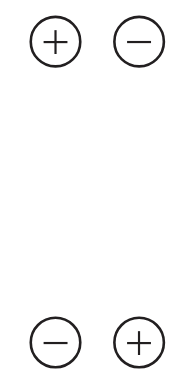
\includegraphics[width=0.3\textwidth]{uni1}
			\caption[]{\label{uni1}}
		\end{subfigure}
		\hfill
		\begin{subfigure}[b]{0.4\textwidth}
			\centering
			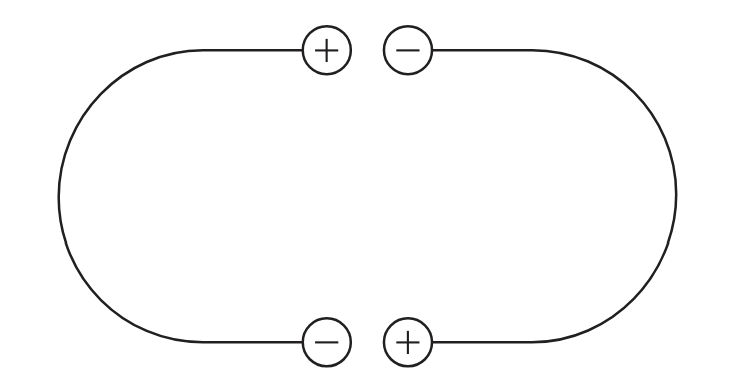
\includegraphics[width=\textwidth]{uni2}	
			\caption[]{\label{uni2}}
		\end{subfigure}
		
		\begin{subfigure}[b]{0.4\textwidth}
			\centering
			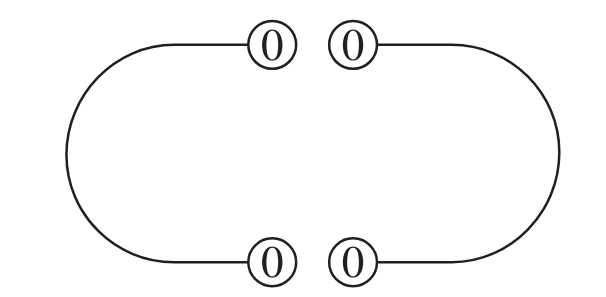
\includegraphics[width=\textwidth]{uni3}	
			\caption[]{\label{uni3}}
		\end{subfigure}
		
		\caption[]{\label{uni}}
	\end{figure}
	
	
	
	\furtherprac{Griffiths 5th ed. Problem 3.5}{There is a variant to the second uniqueness theorem, which states that the electric field is uniquely determined when \(\rho \) is given and either \(V \text { or } \pdv{V}{n} \) is specified on each boundary surface. Prove this.}
	
	\section{The Method of Images}
	
	Suppose a point charge \(q\) is held a distance \(d\) above an infinite grounded conducting plane and we wish to find the potential in the region above the plane. From a mathematical standpoint, this is equivalent to solving the Poisson's equation in the region \(z > 0\), with \(\rho \) corresponds to a single point charge  \(q\) located at \((0,0,d )\), subject to the boundary conditions: 
	\begin{enumerate}
		\item \(V = 0\) when \(z = 0\), and
		\item \(V \rightarrow 0\) for \(x^2 + y^2 + z^2 \gg d^2\).	
	\end{enumerate}
	
	By our clever insights, we see that for the potential created by a pair of opposite charge with \(q\) located at \((0,0,d)\) and \(-q\) located at \((0,0,-d)\) satisfy \(\rho \) in the region \(z > 0\)\footnote{\(\rho \) has to be satisfy since the first uniqueness theorem has the assumption that the charge density throughout the region that we would like to calculate its potential is given. This means that we cannot place image charges in the volume \(\mathcal{V} \) where we are calculating the potential.} as well as all the boundary conditions. Therefore, we can invoke the first uniqueness theorem and claim this potential as our final and only answer.
	
	Since the electric field is just \(\vb{E} = -\grad{V} \), it is also uniquely determined and the force that the real charge experience can be easily calculated as \(\vb{F} = -\frac{1}{4\pi\epsilon_0} \frac{q^2}{(2d)^2} \vu{z}  \) and the energy can be found by integrating the force from infinity to \(d\) which yields \(\int_{\infty}^{d} \frac{1}{4\pi\epsilon_0} \frac{q^2}{(2z)^2} dz = -\frac{1}{4\pi\epsilon_0} \frac{q^2}{4d}  \) which is only half of the energy of a pair of real charge \(q \text{ and }  -q\) separated by a distance \(2d\). This is because there is no electric field in the region \(z < 0\), or equivalently, the image charge can be move for free, since there isn't any electric field to oppose. So the energy becomes \(U = q_{real} V \) and we only need to take into account real charges. 
	
	\begin{example_template}
		\textbf{Example:} \textbf{Griffiths 5rd ed. Example 3.2} \newline \newline
		\textbf{Question:} A point charge q is situated a distance \(a\) from the center of a conducting shell\footnote{A conductor works just as fine here as well. This is because for \(a > R\), the real charge density is zero inside the shell, so the internal field can be found by solving the Laplace's equation with \(\rho = 0\) and subject to the boundary condition of constant potential at the shell. By invoking the first uniqueness theorem, we see that the internal field equals to zero which resembles the case of a conductor is the only answer.} of radius \(R < a\)\footnote{The same can be done for \(R > a\) but we omit here for simplicity.}. Find the potential outside the sphere if it is  \newline a) grounded\footnote{Grounded means \(V = 0 \) relative to infinity, since it is connected to the Earth by a wire, and Earth has infinite capacitance, if we consider the Earth and the sphere as one conductor, we get \(V = 0\) from \(Q = CV\).}, or \newline b) held at potential \(V_0\), or \newline c) isolated with net charge \(Q\). \newline \newline
		\textbf{Solution:} \newline a) The problem is equivalent to solving the Laplace's equation for the region outside the sphere, subject to the boundary conditions:
		
		\begin{enumerate}
			\item V = 0 on the surface of the sphere, and
			\item \(V \rightarrow 0\) for  \(x^2 + y^2 + z^2 \gg R\) 		
		\end{enumerate}
		
		It so happens that the potential created by a point charge \(q' = -\frac{R}{a} q\) located at \(\frac{R^2}{a} \) from the center of the sphere (which always stay inside the sphere since \(R < a\)) together with the real charge satisfies both the boundary conditions and the charge density requirement. Thus, by the first uniqueness theorem, this is our final and only answer. \newline
		
		b) Now the boundary conditions are modified to be:
		
		\begin{enumerate}
			\item \(V = V_0\) on the surface of the sphere, and
			\item \(V \rightarrow 0\) for \(x^2 + y^2 + z^2 \gg R\).	 
		\end{enumerate}
		
		Then since from a) we already know that the potential created by \(q \text{ and } q'\) is zero over the surface of the shell, we only need to add another image charge \(q''\) at the center of the shell (or over the surface of the shell) such that 
		
		\begin{equation}
			V_0 = \frac{1}{4\pi\epsilon_0} \frac{q''}{R}.
		\end{equation}
		
		We see that the potential created by \(q, q' \text{ and } q''\) satisfy both the \(\rho \) requirement as well as the boundary conditions. Therefore, we claim this as our answer. \newline
		
		c) In this part, the boundary conditions are identical to those in b), except for the fact that \(V_0\) is not known but is determined by the total net charge \(Q\). 
		
		To determine the relation between them, we see that since the electric field outside the region which is created by the real point charge and the real induced charge can be regarded as being created by the real point charge and the image charge, the field outside the sphere created by the real induced charge is identical as the field outside the sphere created by the image charge. So we have
		
		\begin{equation}
			\oint _{\mathcal{S} } \vb{E}_{real, induced}  \cdot d\vb{A} = \frac{q_{real, induced}}{\epsilon_0} = \oint _{\mathcal{S} } \vb{E} _{image} \cdot d\vb{A} = \frac{q_{image}}{\epsilon_0} .
		\end{equation}
		
		Therefore we conclude that the image charge is equal to the induced charge. So if the total net charge of the shell is \(Q\), then  we have
		
		\begin{equation}
			Q = q' + q".
		\end{equation}
		
		And the rest is identical to b).
		
	\end{example_template}
	
	\section{Separations of Variables}
	
	The method of separations of variables used for tackling the Laplace's equation is best illustrated with examples.

	\subsection{Cartesian Coordinates}

	In the Cartesian Coordinates, the Laplace's equation reads
		
		\begin{equation}
			\pdv[2]{V}{x} + \pdv[2]{V}{y} + \pdv[2]{V}{z} = 0. 
		\end{equation}
				
		We seek a solution in the form of 
		
		\begin{equation}
			V(x,y) = X(x)Y(y)Z(z).
		\end{equation}
		
		Of course, the solution need not to be in this form. However, if we do find a solution, by any means, that satisfy the Laplace's equation and its boundary conditions, then by the first uniqueness theorem, we know that it must be the only answer. 
		
		Substituting our proposed solution and separating the variables,
		
		\begin{equation}
			\begin{aligned}
				Y \dv[2]{X}{x} + X \dv[2]{Y}{y} + Z \dv[2]{Z}{z} &= 0 \\
				\frac{1}{X} \dv[2]{X}{x} + \frac{1}{Y} \dv[2]{Y}{y} + \frac{1}{Z} \dv[2]{Z}{z} &= 0. 
			\end{aligned}
		\end{equation}
		
		Since we have an equation in the form of \(f(x) + g(y) + h(z) = 0\), the only way the this could possibly be true is that both  \(f,g \text{ and }  z\) must be constant else I could say vary \(x\) while keeping \(y\) constant and the equality wouldn't hold. Thus, we have
		
		\begin{equation}
			\frac{1}{X} \dv[2]{X}{x} = C_1, ~~~\frac{1}{Y} \dv[2]{Y}{y} = C_2 ~~~ \text{ and } ~~~ \frac{1}{Z} \dv[2]{Z}{z} = C_3, ~~~ \text{ with }  C_1 + C_2 + C_3 = 0.
		\end{equation}

	
	\begin{example_template}
		\textbf{Example:} \textbf{Griffths 5rd ed. Example 3.3} \newline \newline
		\textbf{Question:}  Find \(V(x,y)\) in the volume bounded by the metal sheets and infinity as shown in \cref{lap1}.    \newline \newline
		\textbf{Solution:} By symmetry, it is obvious that \(V\) is independent of \(z\), and the boundary conditions are
				
		\begin{enumerate}
			\item \(V = 0\) when \(y = 0 \text { and }  y = a\)
			\item \(V = V_0(y)\) when \(x = 0\)
			\item \(V \rightarrow  0\) as \(x \rightarrow  \infty\).
		\end{enumerate}
		
		With the results derived, we have
		
		\begin{equation}
			\dv[2]{X}{x} = k^2X ~~~ \text{ and } ~~~ \dv[2]{Y}{y} = -k^2Y
		\end{equation}

		where we rewrite the constant \(C_1 \text{ as } k^2\) since \(C_1\) should be positive and  \(C_2\) should be negative, such that \(V(x)\) will admit an exponential decaying function where \(V(x) \rightarrow 0\) as \(x \rightarrow \infty\) and \(V(y)\) will admit a sinusoidal function so that \(V(y)\) will vanish at \(y = 0\) and \(y = a\).            
		
		which gives the solutions
		
		\begin{equation}
			V(x,y) = (A e^{kx} + B e^{-kx} )(C\sin ky+D\cos ky) .
		\end{equation}
		
		Applying the boundary conditions 1 and 3 will left us with 
		
		\begin{equation}
			V(x,y) = C e^{-kx} \sin ky, ~~~ \text{ where } k = \frac{n\pi }{a}. 
		\end{equation}
		
		Since the Laplace's equation is linear, the general solution is the linear combination of all solutions each with different \(n\), so we have 
		
		\begin{equation}
			V(x,y) = \sum_{n=1}^{\infty} C_{n} \sin \frac{n\pi y}{a} e^{-\frac{n\pi x}{a}} .
		\end{equation}
		
		To satisfy the second boundary condition
		
		\begin{equation}
			V(0,y) = \sum_{n=1}^{\infty} C_{n} \sin \frac{n\pi y}{a} = V_0(y) ,
		\end{equation}
		
		we have to rely on the \emph{Fourier's trick} seen in the chapter Fourier series, where we multiply both sides by \(\sin \frac{m\pi y}{a} \) and integrate from \(0 \text { to } a\),
		
		\begin{equation}
			\sum_{n=1}^{\infty} C_{n} \int_{0}^{a} \sin \frac{n\pi y}{a} \sin \frac{m\pi y}{a} dy = \int_{0}^{a} V_0(y) \sin \frac{m\pi y}{a} dy,				 
		\end{equation}
		
		Since 
		
		\begin{equation}
			\int_{0}^{a} \sin \frac{n\pi y}{a} \sin \frac{m\pi y}{a} dy = \begin{cases}
				0 &\text { if } n \neq m, \\ \frac{a}{2} &\text { if } n = m.
			\end{cases},
		\end{equation}
		
		Thus 
		
		\begin{equation}
			C_{n}  = \frac{2}{a} \int_{0}^{a} V_0(y) \sin \frac{n\pi y}{a} dy.  
		\end{equation}
		
		If \(V_0(y) = V_0\), then 
		
		\begin{equation}
			\begin{aligned}
				C_{n} &= \frac{2v_0}{a} \int_{0}^{a} \sin \frac{n\pi y}{a} dy = \frac{2V_0}{n\pi } (1 - \cos n\pi )  \\ 
				&= \begin{cases}
					~ 0 &\text { if } n  \text{ is even}, \\
					\frac{4V_0}{n\pi } &\text { if } n \text{ is odd} .
				\end{cases} 
			\end{aligned}
		\end{equation}
		
		Thus
		
		\begin{equation}
			V(x,y) = \frac{4V_0}{\pi } \sum_{odd~n}^{} \frac{1}{n} \sin \frac{n\pi y}{a}  e^{\frac{-n\pi x}{a}}. 
		\end{equation}
		
		Incidentally, the result can be further simplified by writing \(\sin \frac{in\pi y}{a} \text{ as } \mathfrak{Re} ((-i)e^{\frac{n\pi y}{a} } )  \), then \(V(x,y)\) becomes \(\frac{4V_0 }{\pi } I\), where
		
		\begin{equation}
			I = \mathfrak{Re} ((-i)\sum_{odd~n}^{} \frac{1}{n} (e^{-\frac{\pi (x-iy)}{a} } )^{n}) \end{equation}
		
		Let \(\mathcal{Z} \) to be the exponential, we have
		
		\begin{equation}
			\begin{aligned}
				\sum_{odd~n}^{} \frac{\mathcal{Z} ^{n} }{n} &= \sum_{j=0}^{\infty} \frac{\mathcal{Z} ^{(2j+1)} }{2j+1} = \int_{0}^{\mathcal{Z} } (\sum_{j=1}^{\infty} u^{2j} )du = \int_{0}^{\mathcal{Z} } \frac{du}{1-u^2} \\
				&= \frac{1}{2} \ln (\frac{1+\mathcal{Z} }{1-\mathcal{Z} } ) = \frac{1}{2}  \ln (R e^{i\theta } ) = \frac{1}{2} (\ln R + i\theta )
			\end{aligned}
		\end{equation}
		
		where we have defined \(R e^{i\theta } \text{ as } \frac{1+\mathcal{Z} }{1-\mathcal{Z} } \). So \(I =  \mathfrak{Re}  ((-i)\frac{1}{2} (\ln R + i\theta )) = \frac{\theta }{2}  \). Since 
		\begin{equation}
			\begin{aligned}
				&\frac{1+\mathcal{Z}}{1-\mathcal{Z}}=\frac{1+e^{-\pi(x-i y) / a}}{1-e^{-\pi(x-i y) / a}}=\frac{\left(1+e^{-\pi(x-i y) / a}\right)\left(1-e^{-\pi(x+i y) / a}\right)}{\left(1-e^{-\pi(x-i y) / a}\right)\left(1-e^{-\pi(x+i y) / a}\right)} \\
				& =\frac{1+e^{-\pi x / a}\left(e^{i \pi y / a}-e^{-i \pi y / a}\right)-e^{-2 \pi x / a}}{\left|1-e^{-\pi(x-i y) / a}\right|^2}=\frac{1+2 i e^{-\pi x / a} \sin (\pi y / a)-e^{-2 \pi x / a}}{\left|1-e^{-\pi(x-i y) / a}\right|^2},
			\end{aligned}
		\end{equation}
		
		so
		
		\begin{equation}
			\tan \theta=\frac{2 e^{-\pi x / a} \sin (\pi y / a)}{1-e^{-2 \pi x / a}}=\frac{2 \sin (\pi y / a)}{e^{\pi x / a}-e^{-\pi x / a}}=\frac{\sin (\pi y / a)}{\sinh (\pi x / a)}. 
		\end{equation}
		\todo{why can we ensure that the denominator is real and why did we take the absolute value?}
		
		
		Therefore 
		\begin{equation}
			I=\frac{1}{2} \tan ^{-1}\left(\frac{\sin (\pi y / a)}{\sinh (\pi x / a)}\right), \text { and } \quad V(x, y)=\frac{2 V_0}{\pi} \tan ^{-1}\left(\frac{\sin (\pi y / a)}{\sinh (\pi x / a)}\right) .
		\end{equation}  
		
	\end{example_template}
	
	\begin{figure}[H]
		\centering
		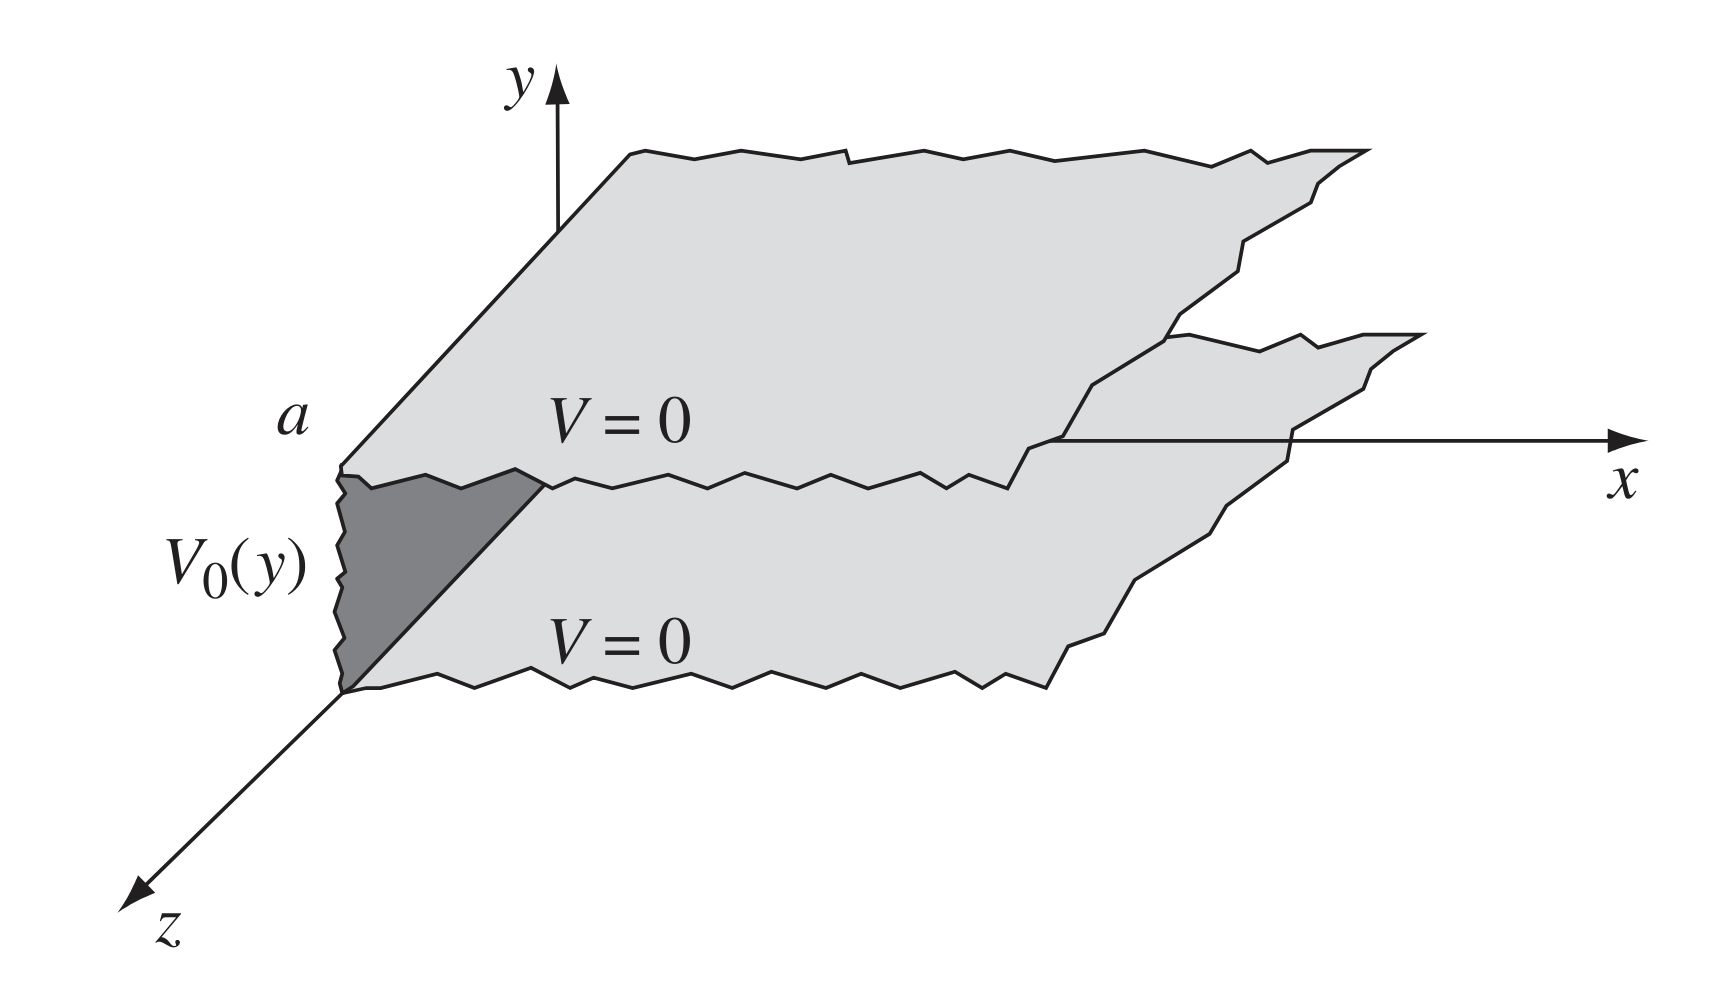
\includegraphics[scale=0.25]{lap1}
		\caption[]{\label{lap1}}
	\end{figure}
	
	
	
	
	
	
	
	\begin{example_template}
		\textbf{Example:} \textbf{Griffths 5rd ed. Example 3.6} \newline \newline
		\textbf{Question:} Find the potential in all space if \(V_0(\theta )\) is specified on a spherical shell of radius \(R\) .  \newline \newline
		\textbf{Solution:}  Since \(V\) is independent of \(\phi \), the Laplace's equation reads 
		
		\begin{equation}
			\pdv{r} (r^2 \pdv{V}{r} ) + \frac{1}{\sin \theta } \pdv{\theta } (\sin \theta \pdv{V}{\theta } ) = 0.
		\end{equation}
		
		Substituting \(V(r,\theta ) = R(r)\Theta (\theta )\) and separating the variables, we have 
		
		\begin{equation}
			\frac{1}{R} \dv{r} (r^2 \dv{R}{r} ) = l(l+1) ~~~ \text{ and } ~~~ \frac{1}{\Theta \sin \theta } \dv{\theta } (\sin \theta \dv{\Theta }{\theta } ) = -l(l+1)	
		\end{equation}
		
		where we have written the separation constant as \(l(l+1)\) where \(l\) is an positive integer, or else the solution would not be physical on the \(z\) axis as the series solution to the angular differential equation would not converge for \(\theta = 0 \text { or }  \pi \) explained \href{https://jfoadi.me.uk/documents/lecture_mathphys2_08.pdf}{here}.
		
		For the radial ordinary differential equation, the general solution has the form
		
		\begin{equation}
			R(r) = Ar^{l} + \frac{B}{r^{l+1} } .
		\end{equation}
		
		While for the angular ordinary differential equation, the general solutions are Legendre polynomials in the variable \(\cos \theta \), where 
		
		\begin{equation}
			P_{l}(x) = \frac{1}{2^{l} l!} (\dv{x} )^{l} (x^2 - 1)^{l} . 
		\end{equation}
		
		The first few Legendre Polynomials are \(P_0(x) = 1, ~P_1(x) = x \text{ and } P_2(x) = \frac{3x^2 - 1}{2} \). Also, with the factor \(\frac{1}{2^{l} l!} \) introduced, we have \(P_{l} (1) = 1\).  
		
		However since the angular differential equation is second order, it should possess two independent solutions for every value of \(l\). It turns out that the other solution blow up at the \(z\) axis anyways and is eliminated by initial or boundary conditions such that the coefficient introduced due to the linearity of the differential equation becomes zero.
		
		From the linearity of the Laplace's equation, the general solution is
		
		\begin{equation}
			\sum_{l=0}^{\infty} (A_{l} r^{l} + \frac{B_{l} }{r^{l+1} } )P_{l} (\cos \theta). \label{sphlap1} 
		\end{equation}
		
		For the region inside the shell, we immediately see that \(B_{l} = 0\) otherwise the potential would blow up at the origin. Also, we require that 
		
		\begin{equation}
			V(R,\theta ) = \sum_{l=0}^{\infty} A_{l} R^{l} P_{l} (\cos \theta ) = V_{0} (\theta )
		\end{equation}
		
		We again use the \emph{Fourier's trick} , but this time we multiply by \(P_{l'} (\cos \theta )\) and use the fact that 
		
		\begin{equation}
			\begin{aligned}
				\int_{-1}^{1} P_{l} (x) P_{l'} (x) dx &= \int_{0}^{\pi } P_{l} (\cos \theta ) P_{l'} (\cos \theta ) \sin \theta d\theta \\ &= \begin{cases}
					~~~ 0 &\text { if } l'\neq l, \\ \frac{2}{2l+1} &\text { if } l' = l.
				\end{cases}
			\end{aligned}
		\end{equation}
		
		Thus by similar means as the previous example, we get
		
		\begin{equation}
			A_{l} = \frac{2l+1}{2R^{l} } \int_{0}^{\pi } V_{0} (\theta ) P_{l} (\cos \theta ) \sin \theta d\theta 
		\end{equation}
		
		The integrals can be difficult to evaluate and in practice it is often easier to solve for \(A_{l} \) \emph{by eyeball}. For example, if \(V_0(\theta ) = k\sin ^2(\frac{\theta }{2} )\), then we can rewrite this as
		
		\begin{equation}
			V_0(\theta ) = \frac{k}{2} (1-\cos \theta ) = \frac{k}{2} (P_0(\cos \theta ) - P_1(\cos \theta )).
		\end{equation}
		
		So we immediately read off from \cref{sphlap1} that \(A_0 = \frac{k}{2} \text{ and }  A_1 = -\frac{k}{2R} \) and
		
		\begin{equation}
			V(r,\theta )  = \frac{k}{2} (1 - \frac{r}{R} \cos \theta ).
		\end{equation}	
		
		And if \(V_0(\theta) = k\cos (3 \theta)\), then we can rewrite this as
		
		\begin{equation}
			V_0(\theta) = k(4\cos ^3 \theta - 3\cos \theta) = \frac{k}{5} (8P_3 (\cos \theta) - 3P_1(\cos \theta)).
		\end{equation}
		
		So we can find that \(A_1 = -\frac{3k}{5R} \text{ and } A_3 = \frac{8k}{5R^3} \) and 
		
		\begin{equation}
			V(r,\theta) = \frac{kr\cos \theta}{5R} (4(\frac{r}{R} )^2(5\cos ^2 \theta-3)-3). 
		\end{equation}
		
		
	\end{example_template}
	
	\begin{example_template}
		\textbf{Example:} \textbf{Griffths 5rd ed. Example 3.8} \newline \newline
		\textbf{Question:} Find the potential in the region outside of a uncharged metal sphere of radius \(R\) placed in an other wise unifrom electric field \(\vb{E} = E_0 \vu{z} \).   \newline \newline
		\textbf{Solution:}  Since \(V\) does not goes to zero at infinity, we redefine the potential to be zero at the surface of the sphere (since it is an equipotential surface). Then the boundary conditions becomes
		
		\begin{enumerate}
			\item \(V = 0 \text { when } r = R\),
			\item \(V \rightarrow -E_0z = -E_0r\cos \theta \text { for } r \gg R.\) 
		\end{enumerate}
		
		Applying the first boundary condition gives
		
		\begin{equation}
			V(r,\theta ) = \sum_{l=0}^{\infty} A_{l} (r^{l}  - \frac{R^{2l+1} }{r^{l+1} } ) P_{l} (\cos \theta ). 			
		\end{equation}
		
		And the second boundary condition requires that 
		
		\begin{equation}
			\sum_{l=0}^{\infty} A_{l} r^{l} P_{l} (\cos \theta ) = -E_0 r\cos \theta .  
		\end{equation}
		
		Thus, we read off \(A_1 = -E_0\) and all other \(A_{l}\)s are zero and the potential is 
		
		\begin{equation}
			V(r,\theta ) = -E_0 (r-\frac{R^3}{r^2} ) \cos \theta 
		\end{equation}
		
		where the first term is due to the external field and the second term is contributed by the induced charge.
		
		The induced charge density can be calculated by 
		
		\begin{equation}
			\sigma (\theta ) = -\epsilon_0 \eval{\pdv{V}{r} }_{r=R}^{} = 3 \epsilon_0	E_0 \cos \theta  
		\end{equation}
		
	\end{example_template}
	
	\begin{example_template}
		\textbf{Example:} \textbf{Griffths 5rd ed. Example 3.9} \newline \newline
		\textbf{Question:} A specified charge density \(\sigma_0(\theta)\) is glued over the surface of a spherical shell of radius \(R\). Find the resulting potential inside and outside the sphere without using \cref{potential}.  \newline \newline
		\textbf{Solution:}  
	\end{example_template}
	
	The success of the method of separation of variables hinges on two extraordinary properties of the separable solutions, namely the completeness and orthogonality. A set of functions \(f_{n} (y)\) is said to be complete if any other function \(f(y)\) can be expressed as a linear combination of them, \ie 
	
	\begin{equation}
		f(y) = \sum_{n=1}^{\infty} C_{n} f_{n} (y). 
	\end{equation}
	
	For example, the functions \(\sin \frac{n\pi y}{a}\), where \(n\) are positive integers are complete over the interval \(0~\le~y\le~a\) as guaranteed by Dirichlet's theorem. Also, any \(n\)th order polynomials can be expressed as the linear combination of the first \(n+1\) Legendre's polynomials, so the set of functions \(P_{l} (x)\) is complete for polynomials.
	
	Orthogonality, on the other hand, means that the integral of the product of any two distinct members of the set is zero, \ie 
	\begin{equation}
		\int_{0}^{a} f_{n} (y) f_{n'} (y) dy = 0 \text { for }  n' \neq n. 
	\end{equation}
	
	It is this property that allows us to perform the \emph{Fourier's trick}.

	
	
	
	
	
	
	
	
	
	
\end{document}

